\documentclass{article}
\usepackage[utf8]{inputenc}
\usepackage{amssymb}
\usepackage{enumitem}
\usepackage{array}
\usepackage{tikz}
\usetikzlibrary{automata, positioning, arrows.meta}
\usepackage[fleqn]{amsmath}
\usepackage[top=2cm, bottom=2cm, left=2.5cm, right=2.5cm]{geometry}

\title{Automátas y Lenguajes Formales 25-2 \\ Tarea 3: Autómatas Finitos}
\author{Hernández Vázquez Carlos Arturo }
\date{Martes 18 de Marzo del 2025}

\begin{document}

\maketitle

\begin{enumerate}
    \item (1pt) Sean $x,y \in \Sigma ^*$. Pruebe la siguiente propiedad de la función de transición extendida para AFD:
    $$\delta^*(q,xy) = \delta^*(\delta^*(q,x),y)$$
    Concluya a partir de esto la definición alternativa de $\delta^*$, es decir, que si $a \in \Sigma$ y $x \in \Sigma^*$, entonces $$\delta^*(q,ax) = \delta^*(\delta(q,a),x)$$

    \textbf{Demostración por inducción sobre $y$:}
    $$\underline{\text{Caso Base}}$$ Sea $y = \epsilon.~ \text{Por demostrar: }$
    $$\delta^*(q,x\epsilon) = \delta^*(\delta^*(q,x),\epsilon)$$\\
    Por definición de $\delta^*$ (caso base de la definición), $$\delta^*(q,x \epsilon) = \delta^*(q,x) =\delta^*(\delta^*(q,x),\epsilon)$$

    $$\underline{\text{Hipotesis de Inducción}}$$ Supongamos que $\forall x,y \in \Sigma^*$ se cumple que $$\delta^* (q,xy) = \delta^*(\delta^*(q,x),y)$$
    
    $$\underline{\text{Paso Inductivo}}$$ Sea $ y = ya,~a \in \Sigma.$ Por demostrar
    $$\delta^* (q,xya) = \delta^*(\delta^*(q,x),ya)$$
    \begin{align*}
    \delta^*(q,xya) &= \delta (\delta^*(q,xy),a) --- \text{ def. de } \delta^* \\
      &= \delta (\delta^*(\delta^*(q,x),y),a) --- \text{ Hip. ind.} \\
      &= \delta^*(\delta^*(q,x),ya) --- \text{ def de } \delta^* \\
    \end{align*}
    $$\boxed{\therefore \delta^*(q,xy) = \delta^*(\delta^*(q,x),y)}$$

    Con la anterior tenemos:
    \begin{align*}
    \delta^*(q,ax) &= \delta^*(\delta^*(q,a),x) --- a \in \Sigma \land a \in \Sigma^* \\
      &= \delta^*(\delta(q,a),x) --- a \in \Sigma \land a \in \Sigma^* \text{ (no es necesaria la } \delta^*)
    \end{align*}:q
    $$\boxed{\therefore \delta^*(q,ax) = \delta^*(\delta(q,a),x)}$$
    
    \item (3 pts.) Diseñar AFD's para que reconozcan cada uno de los siguientes lenguajes:

    \textbf{NOTA:} En los automas construidos se omiten estados de error, y se da por hecho que si un estado no cuenta con una transción en particular, el automata se detiene y no acepta la cadena.  

    \begin{enumerate}
        \item El lenguaje sobre el alfabeto $\{0, 1\}$ en el que todas las cadenas \textbf{no} terminan con $01$

        \begin{center}
            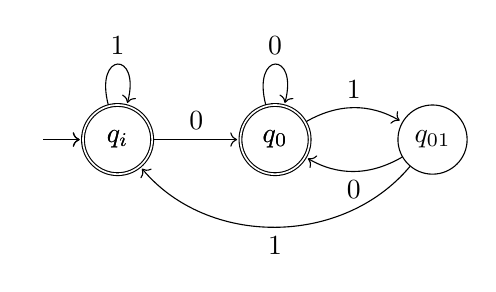
\begin{tikzpicture}[shorten >=1pt, node distance=2cm, on grid, auto]
                \tikzset{initial text={}}
                
                % INITIAL STATE
                \node[state, initial] (qi) {$q_i$}; 
                

                % STATES
                \node[state] (q0) [right=of qi] {$q_0$}; 
                \node[state] (q01) [right=of q0] {$q_{01}$}; 

                % TRANSITIONS
                \path[->]
                    (qi) edge node {0} (q0) 
                    (qi) edge [loop above] node {1} (qi) 
                    (q0) edge [loop above] node {0} (q0)
                    (q0) edge [bend left] node {1} (q01)
                    (q01) edge [bend left] node {0} (q0)
                    (q01) edge [bend left=50] node {1} (qi);
            
                % ACCEPTING STATE
                \node[state, accepting] at (qi) {$q_{i}$};
                \node[state, accepting] at (q0) {$q_{0}$};
                
                \draw[->] ([xshift=-.5cm] qi.west) -- (qi.west) node[midway, above] {};
            
            \end{tikzpicture}
        \end{center}
        
        \item $L = \{w \in \{\ 0,1\}^* \mid |w| = 4n \text{ y } w \text{ contiene ceros en las posiciones pares} \}$ Además, mostrar mediante la función $\delta^*$ la aceptación de la cadena $10001010$.

        \begin{center}
            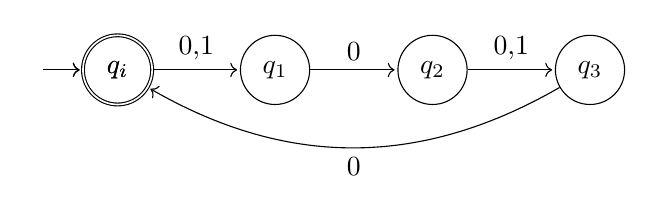
\begin{tikzpicture}[shorten >=1pt, node distance=2cm, on grid, auto]
                \tikzset{initial text={}}
                
                % INITIAL STATE
                \node[state, initial] (qi) {$q_i$}; 
                
                % STATES
                \node[state] (q1) [right=of qi] {$q_1$}; 
                \node[state] (q2) [right=of q1] {$q_{2}$}; 
                \node[state] (q3) [right=of q2] {$q_{3}$}; 

                % TRANSITIONS
                \path[->]
                    (qi) edge node {0,1} (q1) 
                    (q1) edge node {0} (q2) 
                    (q2) edge node {0,1} (q3)
                    (q3) edge [bend left] node {0} (qi);
            
                % ACCEPTING STATE
                \node[state, accepting] at (qi) {$q_{i}$};
                
                \draw[->] ([xshift=-.5cm] qi.west) -- (qi.west) node[midway, above] {};
            
            \end{tikzpicture}
        \end{center}
        Tenemos:
        \begin{align*}
            &\delta^*(q_i,10001010) = \delta(\delta^*(q_i,1000101),0)\\
            &\delta^*(q_i,1000101) = \delta(\delta^*(q_i,100010),1)\\
            &\delta^*(q_i,100010) = \delta(\delta^*(q_i,10001),0)\\
            &\delta^*(q_i,10001) = \delta(\delta^*(q_i,1000),1)\\
            &\delta^*(q_i,1000) = \delta(\delta^*(q_i,100),0)\\
            &\delta^*(q_i,100) = \delta(\delta^*(q_i,10),0)\\
            &\delta^*(q_i,10) = \delta(\delta^*(q_i,1),0)\\
            &\delta^*(q_i,1) = \delta(\delta^*(q_i,\varepsilon),1)\\
            &\delta^*(q_i,\varepsilon) = q_i\\
        \end{align*}

        Sustituyendo:
        \begin{align*}
            &\delta^*(q_i,1) = \delta(q_i,1)\\
            &\delta^*(q_i,10) = \delta(q_1,0)\\
            &\delta^*(q_i,100) = \delta(q_2,0)\\
            &\delta^*(q_i,1000) = \delta(q_3,0)\\
            &\delta^*(q_i,10001) = \delta(q_i,1)\\
            &\delta^*(q_i,100010) = \delta(q_1,0)\\
            &\delta^*(q_i,1000101) = \delta(q_2,1)\\
            &\delta^*(q_i,10001010) = \delta(q_3,0) = q_i\\
        \end{align*}
        \underline{Así, la cadena \textit{10001010} \textbf{si }es aceptada por al autómata.}
         
        \newpage

        \item $L = \{ w \in \{ 0,1 \}^* \mid 00 \text{ no es subcadena de } w \text{ y } w \text{ termina con } 01 \}$
 
        \begin{center}
            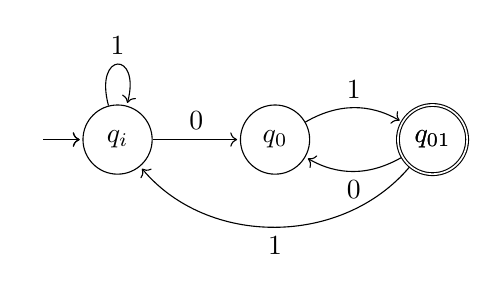
\begin{tikzpicture}[shorten >=1pt, node distance=2cm, on grid, auto]
                \tikzset{initial text={}}
                
                % INITIAL STATE
                \node[state, initial] (qi) {$q_i$}; 
                
                % STATES
                \node[state] (q0) [right=of qi] {$q_0$}; 
                \node[state] (q01) [right=of q0] {$q_{01}$}; 

                % TRANSITIONS
                \path[->]
                    (qi) edge node {0} (q0) 
                    (qi) edge [loop above] node {1} (qi) 
                    (q0) edge [bend left] node {1} (q01) 
                    (q01) edge [bend left] node {0} (q0)
                    (q01) edge [bend left=50] node {1} (qi);
            
                % ACCEPTING STATE
                \node[state, accepting] at (q01) {$q_{01}$};
                
                \draw[->] ([xshift=-.5cm] qi.west) -- (qi.west) node[midway, above] {};
            
            \end{tikzpicture}
        \end{center}

        \item El lenguaje sobre el alfabeto $\{a,b\}$ tal que las cadenas inician con $bbab$ o si inician con una $a$, entonces terminan en $b$.

        \begin{center}
            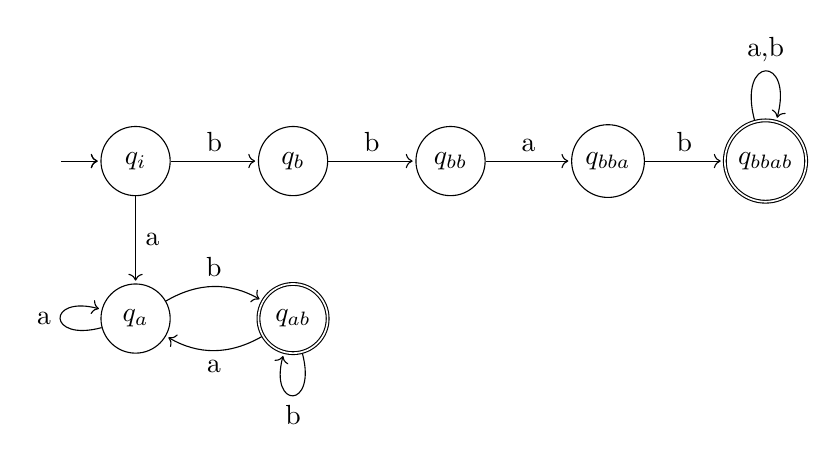
\begin{tikzpicture}[shorten >=1pt, node distance=2cm, on grid, auto]
                \tikzset{initial text={}}
                
                % INITIAL STATE
                \node[state, initial] (qi) {$q_i$}; 
                
                % STATES
                \node[state] (qb) [right=of qi] {$q_b$}; 
                \node[state] (qbb) [right=of qb] {$q_{bb}$}; 
                \node[state] (qbba) [right=of qbb] {$q_{bba}$}; 
                \node[state, accepting] (qbbab) [right=of qbba] {$q_{bbab}$}; 
                \node[state] (qa) [below=of qi] {$q_a$};
                \node[state, accepting] (qab) [right=of qa] {$q_{ab}$};

                % TRANSITIONS
                \path[->]
                    (qi) edge node {b} (qb) 
                    (qi) edge node {a} (qa) 
                    (qa) edge [bend left] node {b} (qab)
                    (qa) edge [loop left] node {a} (qa)
                    (qab) edge [bend left] node {a} (qa)
                    (qab) edge [loop below] node {b} (qab)
                    (qb) edge node {b} (qbb) 
                    (qbb) edge node {a} (qbba) 
                    (qbba) edge node {b} (qbbab) 
                    
                    (qbbab) edge [loop above] node {a,b} (qbbab);
            
                
                \draw[->] ([xshift=-.5cm] qi.west) -- (qi.west) node[midway, above] {};
            
            \end{tikzpicture}
        \end{center}

        \item $L = \{ w \in \{0,1\}^* \mid |w| = 3n \text{ con n} > 0 \text{ y cada bloque de 3 símbolos consecutivos de } w \text{ tiene la subcadena } 01 \}$
        Por ejemplo, las siguientes cadenas pertenecen a $L$: $001, 010, 101, 011, 001101, 101001$, y las siguientes no: $111, 000, 0111, 10100, 010111$.

        \begin{center}
            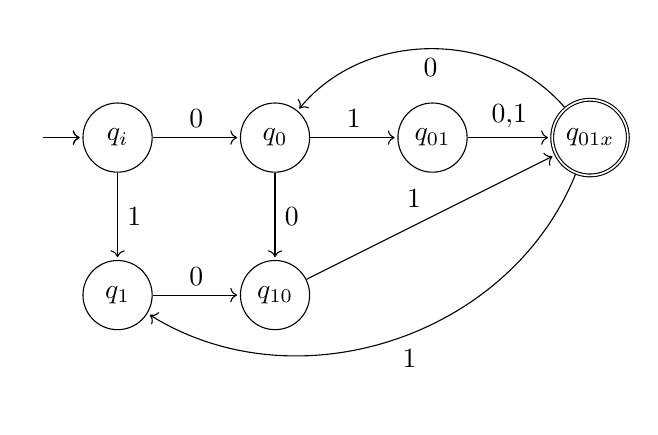
\begin{tikzpicture}[shorten >=1pt, node distance=2cm, on grid, auto]
                \tikzset{initial text={}}
                
                % INITIAL STATE
                \node[state, initial] (qi) {$q_i$}; 
                
                % STATES
                \node[state] (q0) [right=of qi] {$q_0$}; 
                \node[state] (q01) [right=of q0] {$q_{01}$}; 
                \node[state, accepting] (q01x) [right=of q01] {$q_{01x}$}; 
                \node[state] (q1) [below=of qi] {$q_1$};
                \node[state] (q10) [right=of q1] {$q_{10}$};

                % TRANSITIONS
                \path[->]
                    (qi) edge node {0} (q0) 
                    (qi) edge node {1} (q1) 
                    (q0) edge node {1} (q01)
                    (q0) edge node {0} (q10)
                    (q01) edge node {0,1} (q01x)
                    (q01x) edge [bend right=50] node {0} (q0)
                    (q01x) edge [bend left=50] node {1} (q1)
                    (q1) edge node {0} (q10)
                    (q10) edge node {1} (q01x);
                
                \draw[->] ([xshift=-.5cm] qi.west) -- (qi.west) node[midway, above] {};
            
            \end{tikzpicture}
        \end{center}

        \item El lenguaje sobre el alfabeto $\{a,b\}$ cuyas cadenas tienen longitud par pero no contienen a la subcadena $bb$.
        
        \begin{center}
            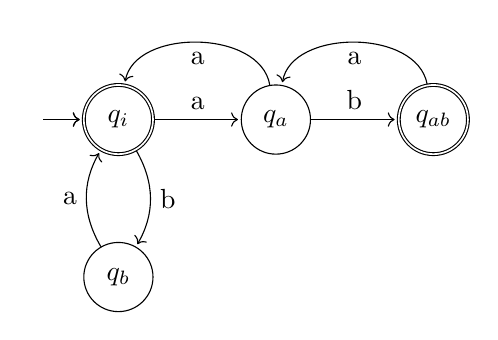
\begin{tikzpicture}[shorten >=1pt, node distance=2cm, on grid, auto]
                \tikzset{initial text={}}
                
                % INITIAL STATE
                \node[state, initial, accepting] (qi) {$q_i$}; 
                
                % STATES
                \node[state] (qa) [right=of qi] {$q_a$}; 
                \node[state, accepting] (qab) [right=of qa] {$q_{ab}$}; 
                \node[state] (qb) [below=of qi] {$q_{b}$};

                % TRANSITIONS
                \path[->]
                    (qi) edge node {a} (qa) 
                    (qa) edge node {b} (qab) 
                    (qi) edge [bend left] node {b} (qb)
                    (qab) edge [bend right=80] node {a} (qa)
                    (qa) edge [bend right=80] node {a} (qi)
                    (qb) edge [bend left] node {a} (qi);
                
                \draw[->] ([xshift=-.5cm] qi.west) -- (qi.west) node[midway, above] {};
            
            \end{tikzpicture}
        \end{center}
    \end{enumerate}
    \newpage
    \item (3 pts) Para el autómata siguiente, describir informalmente el lenguaje aceptado par $M$ y demostrar por inducción sobre la longitud de una cadena que la descripción es correcta.
    
    \begin{table}[h]
        \centering
        \begin{tabular}{c c| c | c}
            $M:$ & $\delta$ & $a$ & $b$ \\
            \hline
            \textit{inicial, final} & $q_0$ & $q_1$ & $q_0$ \\
            \textit{final} & $q_1$ & $q_2$ & $q_0$ \\
            & $q_2$ & $q_2$ & $q_2$
        \end{tabular}
    \end{table}
    \textbf{Descripción del leguaje aceptado}: \\
    El autómata acepta cadenas formadas por $a$'s y/o $b$'s, o incluso la cadena vacía, pero con la condición de que la subcadena $aa$ no esté presente.
    
    \textbf{Demostración por inducción sobre $|w|$}
    
    $$\underline{\text{Caso Base}}$$  
    Sea $w = \varepsilon,$ tal que $|w| = |\varepsilon| = 0$. Por demostrar: $$\text{La cadena $\varepsilon$ es aceptada por el autómata}$$

    Dado que $q_0$ es un estado final, es evidente que $\varepsilon$ es aceptada y la descripción se cumple.
    
    $$\underline{\text{Hipótesis de Inducción}}$$
    $$\text{Toda cadena w, con $|w| = n$, que no contenga la subcadena $aa$ es aceptada por $M$.}$$
    $$\text{Es decir, la cadena es aceptada si después de procesarla no quedamos en $q_2$}$$
    
    $$\underline{\text{Paso Inductivo}}$$  
    Sea $w = sx$, con $s \in \Sigma^*,~x \in \Sigma$, tal que $|sx| = n + 1,~ n >0$. Por demostrar: $$\text{La cadena $sx$ es aceptada por el autómata si $sx$ cumple con la descripción dada. }$$

    Por la construcción de la cadena $sx$, sabemos que $|s| = n$. Por la hipótesis de inducción tenemos que $s$ es aceptada por $M$, y por ende, $s$ no contiene la subcadena $aa$.
    
    Por otro lado, si $x = a$ tenemos diferentes casos:
    \begin{enumerate}
        \item $s$ es aceptada y estamos en $q_0$

        La única manera de estar en $q_0$ con $s$ aceptada es cuando el último símbolo visto fue una $b$. Por tanto, al leer una $a$ llegamos a $q_1$. Lo que significa que $sa$ es aceptada y cumple la descripción.
        \item $s$ es aceptada y estamos en $q_1$

        Si estamos en $q_1$ con $s$ aceptada y procesamos una $a$, llegamos a $q_2$, indicando que $sa$ no es aceptada debido a que contiene algua $aa$. Lo anterior refuerza la descripción dada anteriormente sobre las cadenas que son aceptadas: solo las cadenas que no contengan $aa$ serán aceptadas.
    \end{enumerate}

    Ahora, si $x= b$ tenemos casos similares, pero dado que $s$ ya fue aceptada, es decir, no contiene la subcadena $aa$, concatenarle una $b$ al final no generará la subcadena $aa$ de ninguna forma. Entonces la cadena $sb$ es aceptada por $M$.
    
    $$\boxed{\therefore \text{ la descripción dada sobre las cadenas aceptadas por $M$ es correcta.}}$$
    
    Concluimos que:
    
    $$L(M) = \{ w \in \{a,b\}^* \mid w \text{ no contiene la subcadena } aa \}.$$
    \newpage
    \item (2 pts.) Sean $\Sigma = \{a,b\}$ y $L_3 = \mathcal{L}(\alpha)$ donde $\alpha = (a + b)^*(aaa + bbb)(a + b)^*$.
    \begin{enumerate}
        \item Diseña un \textit{AFN $M_3$} (sin $\epsilon$-transiciones) que acepte a $L_3$

        \begin{center}
            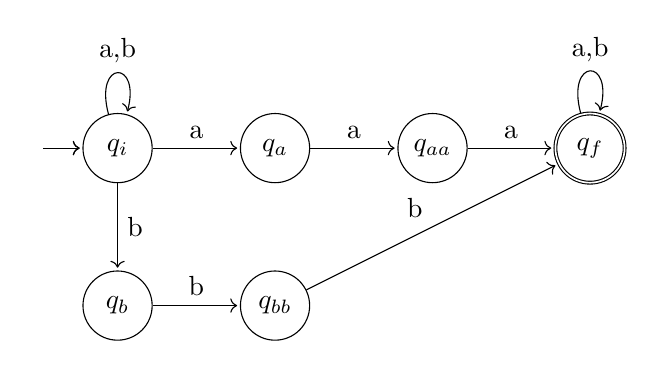
\begin{tikzpicture}[shorten >=1pt, node distance=2cm, on grid, auto]
                \tikzset{initial text={}}
                
                % INITIAL STATE
                \node[state, initial] (qi) {$q_i$}; 
                
                % STATES
                \node[state] (qa) [right=of qi] {$q_a$}; 
                \node[state] (qaa) [right=of qa] {$q_{aa}$}; 
                \node[state, accepting] (qf) [right=of qaa] {$q_{f}$}; 
                \node[state] (qb) [below=of qi] {$q_b$};
                \node[state] (qbb) [right=of qb] {$q_{bb}$};

                % TRANSITIONS
                \path[->]
                    (qi) edge node {a} (qa) 
                    (qi) edge node {b} (qb) 
                    (qi) edge [loop above] node {a,b} (qi) 
                    (qa) edge node {a} (qaa)
                    (qaa) edge node {a} (qf)
                    (qf) edge [loop above] node {a,b} (qf)
                    (qb) edge node {b} (qbb)
                    (qbb) edge node {b} (qf);
                
                \draw[->] ([xshift=-.5cm] qi.west) -- (qi.west) node[midway, above] {};
            
            \end{tikzpicture}
        \end{center}
        
        \item Muestra, usando $\delta^*$, la aceptación de la cadena $abbbb$

        Por un lado tenemos:
        \begin{align*}
        &\delta^*(q_i, abbbb) = \bigcup_{p \in \delta^*(q_i, abbb)} \delta(p,b) \\
        &\delta^*(q_i, abbb) = \bigcup_{p \in \delta^*(q_i, abb)} \delta(p,b)\\
        &\delta^*(q_i, abb) = \bigcup_{p \in \delta^*(q_i, ab)} \delta(p,b)\\
        &\delta^*(q_i, ab) = \bigcup_{p \in \delta^*(q_i, a)} \delta(p,b)\\
        &\delta^*(q_i, a) = \bigcup_{p \in \delta^*(q_i, \epsilon)} \delta(p,a)\\
        \end{align*}

        Sustituyendo de abajo hacia arriba:
        \begin{align*}
        &\delta^*(q_i, a) = \delta(qi,a) = \{q_i, q_a\}\\
        &\delta^*(q_i, ab) = \delta(q_i, b) \cup \delta(q_a,b) = \{q_i, q_b\}\\
        &\delta^*(q_i, abb) = \delta(q_i, b) \cup \delta(q_b,b) = \{q_i, q_b, q_{bb}\}\\
        &\delta^*(q_i, abbb) = \delta(q_i, b) \cup \delta(q_b, b) \cup \delta(q_{bb},b) = \{q_i, q_b, q_{bb},q_f\}\\
        &\delta^*(q_i, abbbb) = \delta(q_i,b) \cup \delta(q_b, b) \cup \delta(q_{bb},b) \cup \delta(q_f,b) = \{q_i, q_b, q_{bb}, q_f\}\\
        \end{align*}

        \textbf{Dado que hemos llegado al estado $q_f$ desde $q_i$, la cadena es aceptada.}
        
        \newpage
        \item Transforma $M_3$ a un \textit{AFD} mediante la construcción de subconjuntos.
        
        Los conjuntos quedan definidos de la siguiente manera:
        
        \begin{table}[h]
        \centering
        \begin{tabular}{c|c|c}
        \hline
         & a & b \\
        \hline
        $\rightarrow q_i$ & $q_i\,q_a$ & $q_i\,q_b$ \\
        $q_a$             & $q_{aa}$   & $\varnothing$ \\
        $q_{aa}$          & $q_f$      & $\varnothing$ \\
        $q_b$             & $\varnothing$ & $q_{bb}$ \\
        $q_{bb}$          & $\varnothing$ & $q_f$ \\
        $*q_f$             & $q_f$      & $q_f$ \\
        \hline
        $\,q_i\,q_a$     & $q_i\,q_a\,q_{aa}$ & $q_i\,q_b$ \\
        $\,q_i\,q_b$     & $q_i\,q_a$         & $q_i\,q_b\,q_{bb}$ \\
        $\,q_i\,q_a\,q_{aa}$ & $q_i\,q_a\,q_{aa}\,q_f$ & $q_i\,q_b$ \\
        $\,q_i\,q_b\,q_{bb}$ & $q_i\,q_a$         & $q_i\,q_b\,q_{bb}\,q_f$ \\
        $*\,q_i\,q_a\,q_{aa}\,q_f$    & $q_i\,q_a\,q_{aa}\,q_f$      & $q_i\,q_b\,q_f$ \\
        $*\,q_i\,q_b\,q_{bb}\,q_f$ & $q_i\,q_a\,q_f$ & $q_i\,q_b\,q_{bb}\,q_f$ \\
        $*\,q_i\,q_b\,q_f$ & $q_i\,q_a\,q_f$         & $q_i\,q_b\,q_{bb}\,q_f$ \\
        $*\,q_i\,q_a\,q_f$ & $q_i\,q_a\,q_{aa}\,q_f$         & $q_i\,q_b\,q_f$ \\
        \hline
        \end{tabular}
        \end{table}

        Así, el autómata queda de la siguiente manera
        \begin{center}
        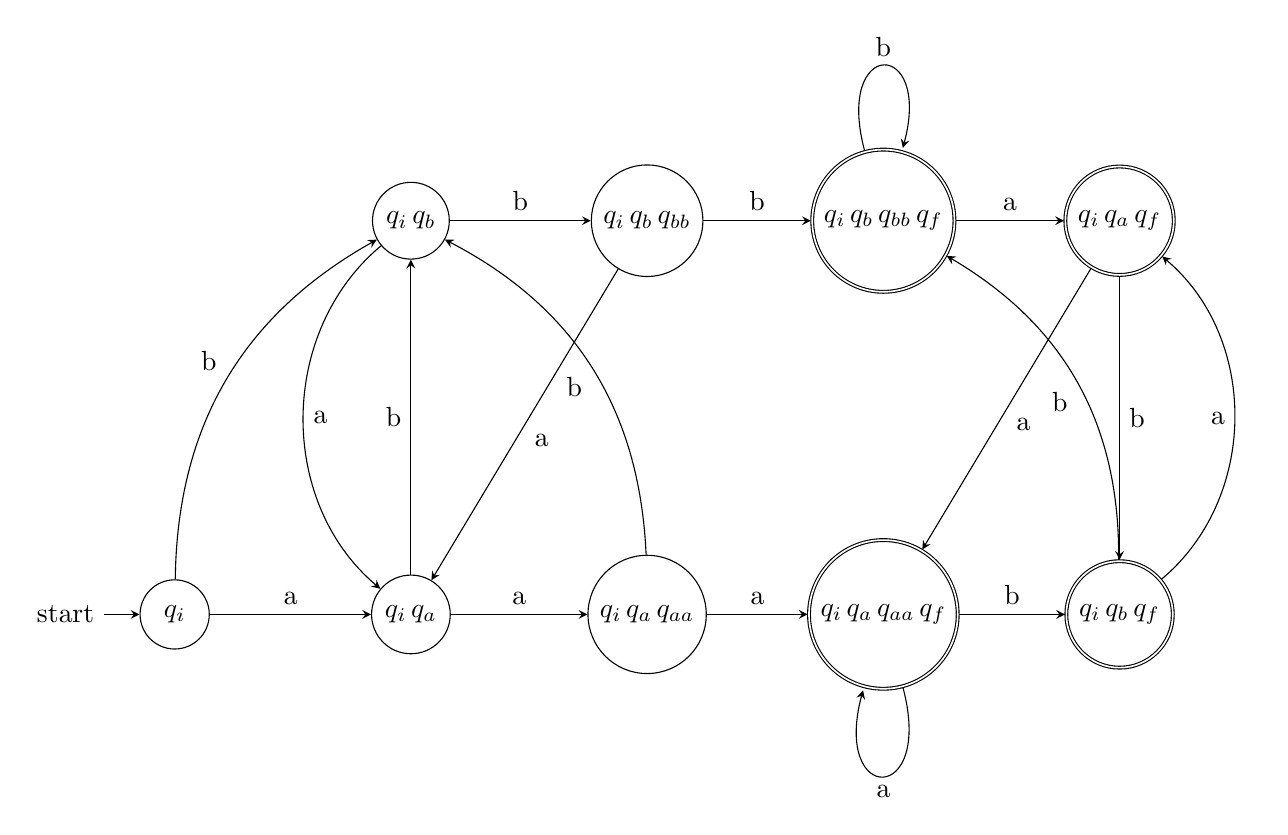
\begin{tikzpicture}[->,>=stealth,node distance=3.2cm,on grid,auto]
            %%% NODOS (estados) %%%
            % Estados “simples”
            \node[state,initial] (qi) {$q_i$};
        
            % Estados “compuestos”
            \node[state] (qiqa)       [right=3cm of qi] {$q_i\,q_a$};
            \node[state] (qiqb)       [above=5cm of qiqa] {$q_i\,q_b$};
            \node[state] (qiqaqaa)    [right=3cm of qiqa] {$q_i\,q_a\,q_{aa}$};
            \node[state] (qiqbqbb)    [right=3cm of qiqb] {$q_i\,q_b\,q_{bb}$};
        
            % Estados compuestos finales
            \node[state,accepting] (qiqaqaaf) [right=3cm of qiqaqaa] {$q_i\,q_a\,q_{aa}\,q_f$};
            \node[state,accepting] (qiqbqbbf) [right=3cm of qiqbqbb] {$q_i\,q_b\,q_{bb}\,q_f$};
            \node[state,accepting] (qiqaqf)   [right=3cm of qiqbqbbf] {$q_i\,q_a\,q_f$};
            \node[state,accepting] (qiqbqf)   [right=3cm of qiqaqaaf] {$q_i\,q_b\,q_f$};
        
            %%% TRANSICIONES %%%
            % Estados simples
            \path
            (qi)   edge node {a} (qiqa)
                   edge [bend left] node {b} (qiqb);
        
            % Estados compuestos
            \path
            (qiqa)       edge node {a} (qiqaqaa)
                         edge node {b} (qiqb)
            (qiqb)       edge [bend right=50] node {a} (qiqa)
                         edge node {b} (qiqbqbb)
            (qiqaqaa)    edge node {a} (qiqaqaaf)
                         edge [bend right] node {b} (qiqb)
            (qiqbqbb)    edge node {a} (qiqa)
                         edge node {b} (qiqbqbbf);
        
            % Estados compuestos finales
            \path
            (qiqaqaaf)   edge [loop below] node {a} (qiqaqaaf)
                         edge node {b} (qiqbqf)
            (qiqbqbbf)   edge node {a} (qiqaqf)
                         edge [loop above] node {b} (qiqbqbbqf)
            (qiqbqf)     edge [bend right=50] node {a} (qiqaqf)
                         edge [bend right] node {b} (qiqbqbbf)
            (qiqaqf)     edge node {a} (qiqaqaaf)
                         edge node {b} (qiqbqf);
        \end{tikzpicture}

        \end{center}
    \end{enumerate}
    \newpage
    \item (3 pts) Sea $M_4$ el autómata siguiente:
    
\begin{center}
    \begin{tabular}{c|c c c}
        & $\varepsilon$ & $a$ & $b$ \\
        \hline
        \textit{inicial} $q_1$ & $\emptyset$ & $\{q_2\}$ & $\emptyset$ \\
        $q_2$ & $\{q_3\}$ & $\{q_2\}$ & $\{q_4\}$ \\
        $q_3$ & $\emptyset$ & $\{q_4\}$ & $\{q_3, q_4\}$ \\
        $q_4$ & $\{q_5\}$ & $\{q_4\}$ & $\emptyset$ \\
        \textit{final} $q5$ & $\emptyset$ & $\emptyset$ & $\emptyset$
    \end{tabular}
\end{center}

    \begin{enumerate}
    
        \item Calcula paso a paso el reconocimiento de las siguientes cadenas y determina si son o no aceptadas: $\delta^*(q_1, abba)$ y $\delta^*(q_1, abab)$
        
        \textbf{Para la cadena $abba$}\\
        Por un lado tenemos:
        \begin{align*}
        &\delta^*(q_1, abba) = Cl_{\varepsilon}(\bigcup_{q' \in \delta^*(q_1, abb)} \delta(q',a)) \\
        &\delta^*(q_1, abb) = Cl_{\varepsilon}(\bigcup_{q' \in \delta^*(q_1, ab)} \delta(q',b)) \\
        &\delta^*(q_1, ab) = Cl_{\varepsilon}(\bigcup_{q' \in \delta^*(q_1, a)} \delta(q',b)) \\
        &\delta^*(q_1, a) = Cl_{\varepsilon}(\bigcup_{q' \in \delta^*(q_1, \varepsilon)} \delta(q',a)) \\
        &\delta^*(q_1, \varepsilon) = Cl_{\varepsilon}(q_1) \\
        \end{align*}
        
        Sustituyendo de abajo hacia arriba:
        \begin{align*}
        &\delta^*(q_1, \varepsilon) = Cl_{\varepsilon}(q_1) = \{q_1\} \\
        &\delta^*(q_1, a) = Cl_{\varepsilon}(\delta(q_1,a)) = Cl_{\varepsilon}(\{q_2\}) = \{q_2, q_3\} \\
        &\delta^*(q_1, ab) = Cl_{\varepsilon}(\bigcup_{q' \in\{q_2, q_3\}}\delta(q',b)) = Cl_{\varepsilon}(\delta(q_2,b) \cup \delta(q_3,b)) = Cl_{\varepsilon}(\{q_3,q_4\}) = \{q_3, q_4, q_5\} \\
        &\delta^*(q_1, abb) = Cl_{\varepsilon}(\bigcup_{q' \in\{q_3, q_4, q_5\}}\delta(q',b)) = Cl_{\varepsilon}(\delta(q_3,b) \cup \delta(q_4,b) \cup \delta(q_5, b)) = Cl_{\varepsilon}(\{q_3,q_4\}) = \{q_3, q_4,q_5\} \\
        &\delta^*(q_1, abba) = Cl_{\varepsilon}(\bigcup_{q' \in\{q_3, q_4, q_5\}}\delta(q',a)) = Cl_{\varepsilon}(\delta(q_3,a) \cup \delta(q_4,a) \cup \delta(q_5, a)) = Cl_{\varepsilon}(\{q_4\}) = \{q_4,q_5\}
        \end{align*}
        \underline{La cadena $abba$ \textbf{si} es aceptada.}\\
        
        \textbf{Para la cadena $abab$}\\
        Por un lado tenemos:
        \begin{align*}
        &\delta^*(q_1, abab) = Cl_{\varepsilon}(\bigcup_{q' \in \delta^*(q_1, aba)} \delta(q',b)) \\
        &\delta^*(q_1, aba) = Cl_{\varepsilon}(\bigcup_{q' \in \delta^*(q_1, ab)} \delta(q',a)) \\
        &\delta^*(q_1, ab) = Cl_{\varepsilon}(\bigcup_{q' \in \delta^*(q_1, a)} \delta(q',b)) \\
        &\delta^*(q_1, a) = Cl_{\varepsilon}(\bigcup_{q' \in \delta^*(q_1, \varepsilon)} \delta(q',a)) \\
        &\delta^*(q_1, \varepsilon) = Cl_{\varepsilon}(q_1) \\
        \end{align*}
        
        Sustituyendo de abajo hacia arriba:
        \begin{align*}
        &\delta^*(q_1, \varepsilon) = Cl_{\varepsilon}(q_1) = \{q_1\} \\
        &\delta^*(q_1, a) = Cl_{\varepsilon}(\delta(q_1,a)) = Cl_{\varepsilon}(\{q_2\}) = \{q_2, q_3\} \\
        &\delta^*(q_1, ab) = Cl_{\varepsilon}(\bigcup_{q' \in\{q_2, q_3\}}\delta(q',b)) = Cl_{\varepsilon}(\delta(q_2,b) \cup \delta(q_3,b)) = Cl_{\varepsilon}(\{q_3,q_4\}) = \{q_3, q_4, q_5\} \\
        &\delta^*(q_1, aba) = Cl_{\varepsilon}(\bigcup_{q' \in\{q_3, q_4, q_5\}}\delta(q',a)) = Cl_{\varepsilon}(\delta(q_3,a) \cup \delta(q_4,a) \cup \delta(q_5, a)) = Cl_{\varepsilon}(\{q_4\}) = \{q_4,q_5\} \\
        &\delta^*(q_1, abab) = Cl_{\varepsilon}(\bigcup_{q' \in\{q_3, q_4,q_5\}}\delta(q',b)) = Cl_{\varepsilon}(\delta(q_4,b) \cup \delta(q_5,b) ) = Cl_{\varepsilon}(\varnothing) = \varnothing
        \end{align*}
        \underline{La cadena $abab$ \textbf{no} es aceptada.}
        
        \item Da una expresión regular que exprese el lenguaje aceptado por el autómata $M_4$
        
        \textbf{Expresión regular:} $a^+b^*(a + b)a^*$

        \item Elimina las transiciones $\varepsilon$ para obtener un AFN $M'_4$ tal que $\mathcal{L}(M_4) = \mathcal{L}(M'_4)$\\
        Autómata con $\varepsilon$-transiciones:
        \begin{center}
            \begin{tikzpicture}[shorten >=1pt, node distance=2cm, on grid, auto]
                \tikzset{initial text={}}
                
                % INITIAL STATE
                \node[state, initial] (q1) {$q_1$}; 
                
                % STATES
                \node[state] (q2) [right=of q1] {$q_2$}; 
                \node[state] (q3) [right=of q2] {$q_3$}; 
                \node[state] (q4) [below=of q3] {$q_4$};
                \node[state, accepting] (q5) [right=of q4] {$q_5$}; 

                % TRANSITIONS
                \path[->]
                    (q1) edge node {a} (q2) 
                    (q2) edge [loop above] node {a} (q2) 
                    (q2) edge node {b} (q4)
                    (q2) edge node {$\epsilon$} (q3)
                    (q3) edge node {a,b} (q4)
                    (q3) edge [loop above] node {b} (q3)
                    (q4) edge node {$\varepsilon$} (q5)
                    (q4) edge [loop below] node {a} (q4);
                
                \draw[->] ([xshift=-.5cm] qi.west) -- (qi.west) node[midway, above] {};
            
            \end{tikzpicture}
        \end{center}
        
        Autómata sin $\varepsilon$-transiciones:\\
        - Tabla con las $\varepsilon$-transiciones de cada estado:
        
        \begin{center}
            \begin{tabular}{c|c}
                & $Cl_{\varepsilon}(q_i)$ \\
                \hline
                $q_1$ & $\{q_1\}$ \\
                $q_2$ & $\{q_2,q_3\}$ \\
                $q_3$ & $\{q_3\}$ \\
                $q_4$ & $\{q_4,q_5\}$ \\
                $q_5$ & $\{q_5\}$ \\
            \end{tabular}
        \end{center}
        Aplicando la nueva delta del AFN definida como: 
        $$\delta(q,a) = \delta^*(q,a) = Cl_{\varepsilon}(\bigcup_{p \in Cl_{\varepsilon}(q)} \delta_{\varepsilon}(p,a))$$

        
        \begin{align*}
        &\delta(q_1, a) = Cl_{\varepsilon}(\bigcup_{p \in Cl_{\varepsilon}(q_1)} \delta_{\varepsilon}(p,a)) = Cl_\varepsilon(\delta_\varepsilon(q_1,a)) = Cl_\varepsilon(\{q_2\}) = \{q_2, q_3\} \\
        &\delta(q_1, b) = Cl_{\varepsilon}(\bigcup_{p \in Cl_{\varepsilon}(q_1)} \delta_{\varepsilon}(p,b)) = Cl_\varepsilon(\delta_\varepsilon(q_1,b)) = Cl_\varepsilon(\varnothing) = \varnothing \\
        &\delta(q_2, a) = Cl_{\varepsilon}(\bigcup_{p \in Cl_{\varepsilon}(q_2)} \delta_{\varepsilon}(p,a)) = Cl_\varepsilon(\delta_\varepsilon(q_2,a)\cup \delta_\varepsilon(q_3, a)) = Cl_\varepsilon(\{q_2,q_4\}) = \{q_2, q_3, q_4, q_5\} \\
        &\delta(q_2, b) = Cl_{\varepsilon}(\bigcup_{p \in Cl_{\varepsilon}(q_2)} \delta_{\varepsilon}(p,b)) = Cl_\varepsilon(\delta_\varepsilon(q_2,b)\cup \delta_\varepsilon(q_3, b)) = Cl_\varepsilon(\{q_3,q_4\}) = \{q_3, q_4, q_5\} \\
        \end{align*}
        \begin{align*}
        &\delta(q_3, a) = Cl_{\varepsilon}(\bigcup_{p \in Cl_{\varepsilon}(q_3)} \delta_{\varepsilon}(p,a)) = Cl_\varepsilon(\delta_\varepsilon(q_3, a)) = Cl_\varepsilon(\{q_4\}) = \{q_4, q_5\} \\
        &\delta(q_3, b) = Cl_{\varepsilon}(\bigcup_{p \in Cl_{\varepsilon}(q_3)} \delta_{\varepsilon}(p,b)) = Cl_\varepsilon(\delta_\varepsilon(q_3, b)) = Cl_\varepsilon(\{q_3,q_4\}) = \{q_3,q_4, q_5\} \\
        &\delta(q_4, a) = Cl_{\varepsilon}(\bigcup_{p \in Cl_{\varepsilon}(q_4)} \delta_{\varepsilon}(p,a)) = Cl_\varepsilon(\delta_\varepsilon(q_4, a)\cup \delta_\varepsilon(q_5,a)) = Cl_\varepsilon(\{q_4\}) = \{q_4, q_5\} \\
        &\delta(q_4, b) = Cl_{\varepsilon}(\bigcup_{p \in Cl_{\varepsilon}(q_4)} \delta_{\varepsilon}(p,b)) = Cl_\varepsilon(\delta_\varepsilon(q_4, b)\cup \delta_\varepsilon(q_5,b)) = Cl_\varepsilon(\varnothing) = \varnothing\\
        &\delta(q_5, a) = Cl_{\varepsilon}(\bigcup_{p \in Cl_{\varepsilon}(q_5)} \delta_{\varepsilon}(p,a)) = Cl_\varepsilon(\delta_\varepsilon(q_5,a)) = Cl_\varepsilon(\varnothing) = \varnothing \\
        &\delta(q_5, b) = Cl_{\varepsilon}(\bigcup_{p \in Cl_{\varepsilon}(q_5)} \delta_{\varepsilon}(p,b)) = Cl_\varepsilon(\delta_\varepsilon(q_5,b)) = Cl_\varepsilon(\varnothing) = \varnothing \\
        \end{align*}
        Con lo anterior se puede construir el siguiente $AFN$ sin $\varepsilon$-transiciones
        \begin{center}
            \begin{tikzpicture}[shorten >=1pt, node distance=2cm, on grid, auto]
                \tikzset{initial text={}}
                
                % INITIAL STATE
                \node[state, initial] (q1) {$q_1$}; 
                
                % STATES
                \node[state] (q2) [right=of q1] {$q_2$}; 
                \node[state] (q3) [right=of q2] {$q_3$}; 
                \node[state] (q4) [below=4cm of q3] {$q_4$};
                \node[state, accepting] (q5) [right=of q4] {$q_5$}; 

                % TRANSITIONS
                \path[->]
                    (q1) edge node {a} (q2) 
                    (q1) edge [bend left=60] node {a} (q3)
                    (q2) edge [loop below] node {a} (q2)
                    (q2) edge node {a,b} (q3)
                    (q2) edge [bend right=15] node {a,b} (q4)
                    (q2) edge node {a,b} (q5)
                    (q3) edge [loop above] node {b} (q3)
                    (q3) edge [bend left=50] node {a,b} (q4)
                    (q3) edge [bend left=50] node {a,b} (q5)
                    (q4) edge node {a} (q5)
                    (q4) edge [loop below] node {a} (q4);
                
                \draw[->] ([xshift=-.5cm] qi.west) -- (qi.west) node[midway, above] {};
            \end{tikzpicture}\\
        \end{center}
        \item Elimina el no-determinismo para encontrar un AFD $M''_4$ tal que $\mathcal{L}(M'_4) = \mathcal{L}(M''_4)$\\
        Los conjuntos quedan definidos de la siguiente manera:
        
        \begin{table}[h]
        \centering
        \begin{tabular}{c|c|c}
        \hline
         & a & b \\
        \hline
        $\rightarrow q_1$ & $q_2\,q_3$ & $\varnothing$ \\
        $q_2$          & $q_2\,q_3\,q_4\,q_5$      & $q_3\,q_4\,q_5$ \\
        $q_3$             & $q_4\,q_5$ & $q_3\,q_4\,q_5$ \\
        $q_4$          & $q_4\,q_5$ & $\varnothing$ \\
        $*q_5$             & $\varnothing$      & $\varnothing$ \\
        \hline
        $q_2\,q_3$             & $q_2\,q_3\,q_4\,q_5$      & $q_3\,q_4\,q_5$ \\
        $*q_2\,q_3\,q_4\,q_5$             & $q_2\,q_3\,q_4\,q_5$      & $q_3\,q_4\,q_5$ \\
        $*q_3\,q_4\,q_5$             & $q_4\,q_5$      & $q_3\,q_4\,q_5$ \\
        $*q_4\,q_5$             & $q_4\,q_5$      & $\varnothing$ \\
        \hline
        \end{tabular}
        \end{table}
        
        \newpage
        Así, el autómata queda de la siguiente manera

\begin{center}
    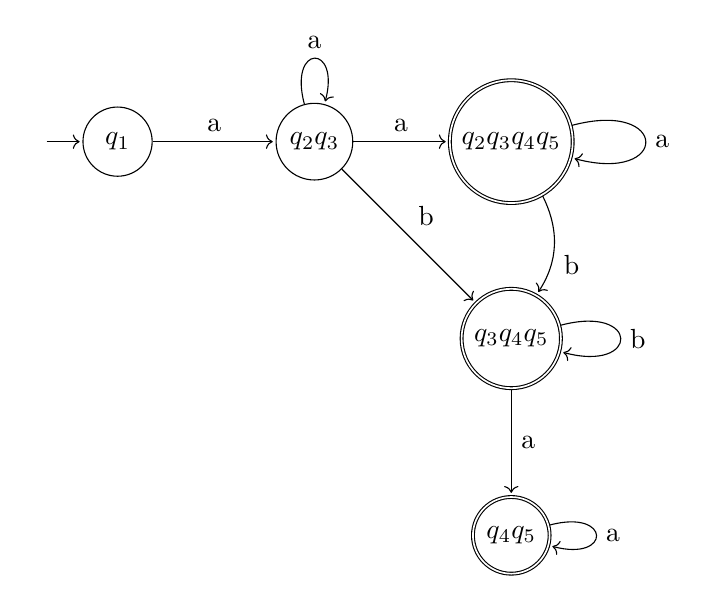
\begin{tikzpicture}[shorten >=1pt, node distance=2.5cm, on grid, auto]
        \tikzset{initial text={}}
        
        % Estados
        \node[state, initial] (q1) {$q_1$}; 
        \node[state] (q23) [right=of q1] {$q_2 q_3$}; 
        \node[state, accepting] (q2345) [right=of q23] {$q_2 q_3 q_4 q_5$};
        \node[state, accepting] (q345) [below=of q2345] {$q_3 q_4 q_5$};
        \node[state, accepting] (q45) [below=of q345] {$q_4 q_5$};
        
        % Transiciones
        \path[->]
            (q1) edge node {a} (q23)
            (q23) edge [loop above] node {a} (q23)
            (q23) edge node {b} (q345)
            (q23) edge node {a} (q2345)
            (q2345) edge [loop right] node {a} (q2345)
            (q2345) edge [bend left] node {b} (q345)
            (q345) edge [loop right] node {b} (q345)
            (q345) edge node {a} (q45)
            (q45) edge [loop right] node {a} (q45);
    \end{tikzpicture}
\end{center}
        
    \end{enumerate}
\end{enumerate}

\end{document}

